% Chapter 1

\chapter{Introduction}\label{ch:introduction}
One of the long-standing goals of humanity is to understand the mechanisms that underlie biological life. The journey towards this end objective requires to solve several fascinating sub-problems: how do biological entities work at the cell level? Which processes determine a particular phenotype? How can we cure diseases? These broad questions require dedicated scientific studies, which necessarily entail analyzing large quantities of data to model complex phenomena. In this sense, the latest technological advancements in collecting, storing, and processing biological information have brought forth unprecedented progress. At the same time, an equal effort has been dedicated to developing computational methodologies that learn difficult biological tasks by extracting useful knowledge from these sheer amounts of data. Among the many, Deep Learning with neural networks \citep{lecun2015naturedeeplearning} has been undoubtedly one of the driving forces in these latest years. As we write this thesis, a Deep Learning model called \emph{AlphaFold} has made a giant leap towards reliably predicting a protein's structure from its sequence of amino acids -- the so-called \emph{protein folding} problem \citep{senior2020alphafold}. With Deep Learning, we can now predict quantum properties of chemical structures within chemical accuracy, being 300k times faster than numerical simulations  \citep{gilmer2017neuralmessagepassing}. A Deep Learning method called \emph{DeepVariant} can reconstruct a true genome sequence from High-Throughput Sequencing data with significantly greater accuracy than previous classical methods \citep{poplin2018deepvariant}. Lastly, Deep Learning has been successfully applied to counter antibiotic resistance by finding chemically different antibiotics from known ones but having the same bactericidal activity \citep{stokes2020deeplearningantibiotic}. All these life sciences problems -- and most life sciences problems more broadly -- share apparent commonalities. One is that each of them concerns a poorly characterized phenomenon, meaning that the biological function that relates the data to the observed outcomes is only partially understood. In this case, Deep Learning is helpful because it shifts the burden of finding a suitable representation of the input data from the user to the modeling machine \citep{bengio2014representationlearning}. In other words, instead of hand-crafting the knowledge required to solve a task, Deep Learning models infer task-specific knowledge from the data themselves. Another commonality regards the nature of the biological datum. Indeed, most biological data are \emph{structured}, meaning that they can be decomposed into a set of entities and relations between them. Structured data in life sciences are ubiquitous: some examples are shown in Figure \ref{fig:biological-data}. Proteins can be thought of as \emph{sequences} of amino acids. Gene ontologies, which describe gene attributes across various species, are organized with \emph{hierarchical} data structures. Molecules are naturally represented as \emph{graphs} where atoms are vertices, and chemical bonds are edges. Clearly, a biological datum taken as a whole has more informative content than its constituents taken in isolation. On the one hand, this superior expressiveness allows devising more effective models of biological processes. On the other hand, working with structured data introduces additional challenges, such as representing them in a computationally efficient way while also preserving their relational nature.

\begin{figure*}[h!]
    \begin{subfigure}[b]{0.32\linewidth}
        \centering
        \resizebox{.9\textwidth}{!}{

\tikzset{every picture/.style={line width=0.75pt}} %set default line width to 0.75pt

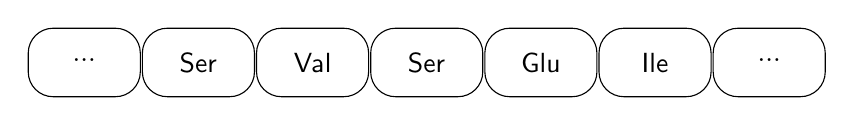
\begin{tikzpicture}[x=0.75pt,y=0.75pt,yscale=-1,xscale=1]
%uncomment if require: \path (0,83); %set diagram left start at 0, and has height of 83


% Text Node
\draw    (78,31) .. controls (78,24.37) and (83.37,19) .. (90,19) -- (120,19) .. controls (126.63,19) and (132,24.37) .. (132,31) -- (132,40) .. controls (132,46.63) and (126.63,52) .. (120,52) -- (90,52) .. controls (83.37,52) and (78,46.63) .. (78,40) -- cycle  ;
\draw (105,35.5) node   [align=left] {\begin{minipage}[lt]{34pt}\setlength\topsep{0pt}
\begin{center}
$\displaystyle \mathsf{Ser}$
\end{center}

\end{minipage}};
% Text Node
\draw    (133,31) .. controls (133,24.37) and (138.37,19) .. (145,19) -- (175,19) .. controls (181.63,19) and (187,24.37) .. (187,31) -- (187,40) .. controls (187,46.63) and (181.63,52) .. (175,52) -- (145,52) .. controls (138.37,52) and (133,46.63) .. (133,40) -- cycle  ;
\draw (160,35.5) node   [align=left] {\begin{minipage}[lt]{34pt}\setlength\topsep{0pt}
\begin{center}
$\displaystyle \mathsf{Val}$
\end{center}

\end{minipage}};
% Text Node
\draw    (188,31) .. controls (188,24.37) and (193.37,19) .. (200,19) -- (230,19) .. controls (236.63,19) and (242,24.37) .. (242,31) -- (242,40) .. controls (242,46.63) and (236.63,52) .. (230,52) -- (200,52) .. controls (193.37,52) and (188,46.63) .. (188,40) -- cycle  ;
\draw (215,35.5) node   [align=left] {\begin{minipage}[lt]{34pt}\setlength\topsep{0pt}
\begin{center}
$\displaystyle \mathsf{Ser}$
\end{center}

\end{minipage}};
% Text Node
\draw    (243,31) .. controls (243,24.37) and (248.37,19) .. (255,19) -- (285,19) .. controls (291.63,19) and (297,24.37) .. (297,31) -- (297,40) .. controls (297,46.63) and (291.63,52) .. (285,52) -- (255,52) .. controls (248.37,52) and (243,46.63) .. (243,40) -- cycle  ;
\draw (270,35.5) node   [align=left] {\begin{minipage}[lt]{34pt}\setlength\topsep{0pt}
\begin{center}
$\displaystyle \mathsf{Glu}$
\end{center}

\end{minipage}};
% Text Node
\draw    (298,31) .. controls (298,24.37) and (303.37,19) .. (310,19) -- (340,19) .. controls (346.63,19) and (352,24.37) .. (352,31) -- (352,40) .. controls (352,46.63) and (346.63,52) .. (340,52) -- (310,52) .. controls (303.37,52) and (298,46.63) .. (298,40) -- cycle  ;
\draw (325,35.5) node   [align=left] {\begin{minipage}[lt]{34pt}\setlength\topsep{0pt}
\begin{center}
$\displaystyle \mathsf{Ile}$
\end{center}

\end{minipage}};
% Text Node
\draw    (23,31) .. controls (23,24.37) and (28.37,19) .. (35,19) -- (65,19) .. controls (71.63,19) and (77,24.37) .. (77,31) -- (77,40) .. controls (77,46.63) and (71.63,52) .. (65,52) -- (35,52) .. controls (28.37,52) and (23,46.63) .. (23,40) -- cycle  ;
\draw (50,35.5) node   [align=left] {\begin{minipage}[lt]{34pt}\setlength\topsep{0pt}
\begin{center}
...
\end{center}

\end{minipage}};
% Text Node
\draw    (353,31) .. controls (353,24.37) and (358.37,19) .. (365,19) -- (395,19) .. controls (401.63,19) and (407,24.37) .. (407,31) -- (407,40) .. controls (407,46.63) and (401.63,52) .. (395,52) -- (365,52) .. controls (358.37,52) and (353,46.63) .. (353,40) -- cycle  ;
\draw (380,35.5) node   [align=left] {\begin{minipage}[lt]{34pt}\setlength\topsep{0pt}
\begin{center}
...
\end{center}

\end{minipage}};


\end{tikzpicture}}
        \caption{Protein sequence.}
        \label{subfig:protein-sequence}
    \end{subfigure}
    \begin{subfigure}[b]{0.36\linewidth}
        \centering
        \resizebox{.9\textwidth}{!}{

\tikzset{every picture/.style={line width=0.75pt}} %set default line width to 0.75pt

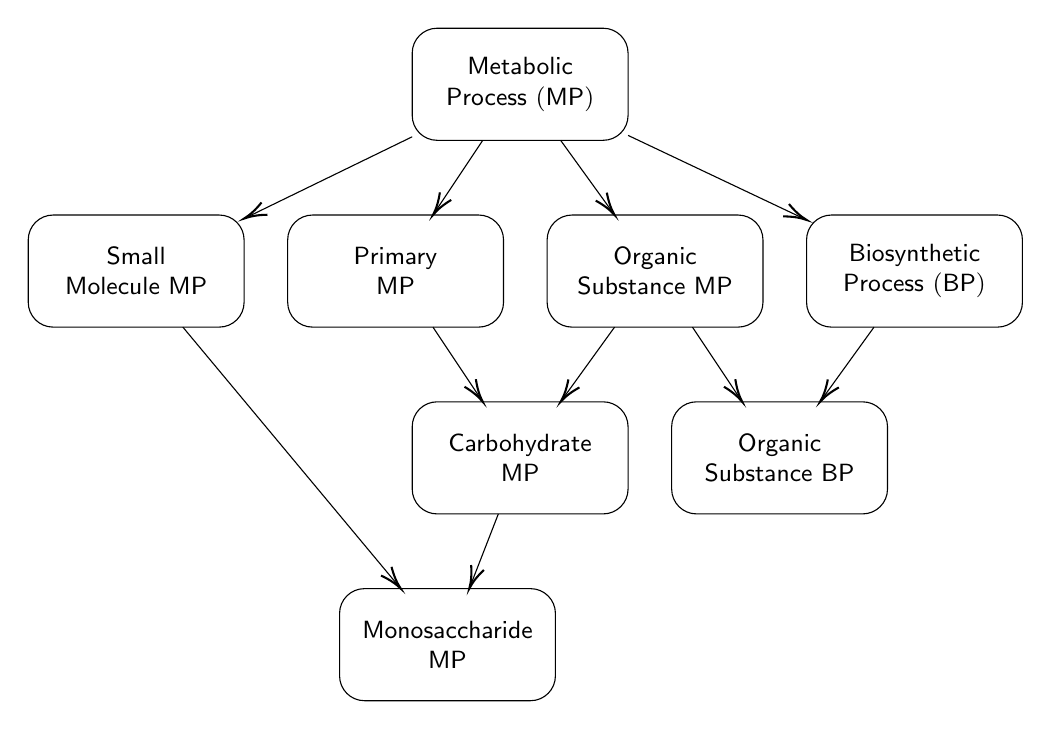
\begin{tikzpicture}[x=0.75pt,y=0.75pt,yscale=-1,xscale=1]
%uncomment if require: \path (0,480); %set diagram left start at 0, and has height of 480


% Text Node
\draw    (236,40) .. controls (236,33.37) and (241.37,28) .. (248,28) -- (328,28) .. controls (334.63,28) and (340,33.37) .. (340,40) -- (340,70) .. controls (340,76.63) and (334.63,82) .. (328,82) -- (248,82) .. controls (241.37,82) and (236,76.63) .. (236,70) -- cycle  ;
\draw (288,55) node  [font=\small] [align=left] {\begin{minipage}[lt]{68pt}\setlength\topsep{0pt}
\begin{center}
$\mathsf{Metabolic}$\\
$\mathsf{Process\ (MP)}$
\end{center}

\end{minipage}};
% Text Node
\draw    (176,130) .. controls (176,123.37) and (181.37,118) .. (188,118) -- (268,118) .. controls (274.63,118) and (280,123.37) .. (280,130) -- (280,160) .. controls (280,166.63) and (274.63,172) .. (268,172) -- (188,172) .. controls (181.37,172) and (176,166.63) .. (176,160) -- cycle  ;
\draw (228,145) node  [font=\small] [align=left] {\begin{minipage}[lt]{68pt}\setlength\topsep{0pt}
\begin{center}
$\mathsf{Primary}$\\
$\mathsf{MP}$
\end{center}

\end{minipage}};
% Text Node
\draw    (301,130) .. controls (301,123.37) and (306.37,118) .. (313,118) -- (393,118) .. controls (399.63,118) and (405,123.37) .. (405,130) -- (405,160) .. controls (405,166.63) and (399.63,172) .. (393,172) -- (313,172) .. controls (306.37,172) and (301,166.63) .. (301,160) -- cycle  ;
\draw (353,145) node  [font=\small] [align=left] {\begin{minipage}[lt]{68pt}\setlength\topsep{0pt}
\begin{center}
$\mathsf{Organic}$
$\mathsf{Substance\ MP}$
\end{center}

\end{minipage}};
% Text Node
\draw    (426,130) .. controls (426,123.37) and (431.37,118) .. (438,118) -- (518,118) .. controls (524.63,118) and (530,123.37) .. (530,130) -- (530,160) .. controls (530,166.63) and (524.63,172) .. (518,172) -- (438,172) .. controls (431.37,172) and (426,166.63) .. (426,160) -- cycle  ;
\draw (478,145) node  [font=\small] [align=left] {\begin{minipage}[lt]{68pt}\setlength\topsep{0pt}
\begin{center}
$\mathsf{Biosynthetic}$\\
$\mathsf{Process\ (BP)}$
\end{center}

\end{minipage}};
% Text Node
\draw    (51,130) .. controls (51,123.37) and (56.37,118) .. (63,118) -- (143,118) .. controls (149.63,118) and (155,123.37) .. (155,130) -- (155,160) .. controls (155,166.63) and (149.63,172) .. (143,172) -- (63,172) .. controls (56.37,172) and (51,166.63) .. (51,160) -- cycle  ;
\draw (103,145) node  [font=\small] [align=left] {\begin{minipage}[lt]{68pt}\setlength\topsep{0pt}
\begin{center}
$\mathsf{Small}$\\
$\mathsf{Molecule\ MP}$
\end{center}

\end{minipage}};
% Text Node
\draw    (236,220) .. controls (236,213.37) and (241.37,208) .. (248,208) -- (328,208) .. controls (334.63,208) and (340,213.37) .. (340,220) -- (340,250) .. controls (340,256.63) and (334.63,262) .. (328,262) -- (248,262) .. controls (241.37,262) and (236,256.63) .. (236,250) -- cycle  ;
\draw (288,235) node  [font=\small] [align=left] {\begin{minipage}[lt]{68pt}\setlength\topsep{0pt}
\begin{center}
$\mathsf{Carbohydrate}$\\
$\mathsf{MP}$
\end{center}

\end{minipage}};
% Text Node
\draw    (361,220) .. controls (361,213.37) and (366.37,208) .. (373,208) -- (453,208) .. controls (459.63,208) and (465,213.37) .. (465,220) -- (465,250) .. controls (465,256.63) and (459.63,262) .. (453,262) -- (373,262) .. controls (366.37,262) and (361,256.63) .. (361,250) -- cycle  ;
\draw (413,235) node  [font=\small] [align=left] {\begin{minipage}[lt]{68pt}\setlength\topsep{0pt}
\begin{center}
$\mathsf{Organic}$\\
$\mathsf{Substance\ BP}$
\end{center}

\end{minipage}};
% Text Node
\draw    (201,310) .. controls (201,303.37) and (206.37,298) .. (213,298) -- (293,298) .. controls (299.63,298) and (305,303.37) .. (305,310) -- (305,340) .. controls (305,346.63) and (299.63,352) .. (293,352) -- (213,352) .. controls (206.37,352) and (201,346.63) .. (201,340) -- cycle  ;
\draw (253,325) node  [font=\small] [align=left] {\begin{minipage}[lt]{68pt}\setlength\topsep{0pt}
\begin{center}
$\mathsf{Monosaccharide}$\\
$\mathsf{MP}$
\end{center}

\end{minipage}};
% Connection
\draw    (236,80.3) -- (156.8,118.83) ;
\draw [shift={(155,119.7)}, rotate = 334.06] [color={rgb, 255:red, 0; green, 0; blue, 0 }  ][line width=0.75]    (10.93,-3.29) .. controls (6.95,-1.4) and (3.31,-0.3) .. (0,0) .. controls (3.31,0.3) and (6.95,1.4) .. (10.93,3.29)   ;
% Connection
\draw    (270,82) -- (247.11,116.34) ;
\draw [shift={(246,118)}, rotate = 303.69] [color={rgb, 255:red, 0; green, 0; blue, 0 }  ][line width=0.75]    (10.93,-3.29) .. controls (6.95,-1.4) and (3.31,-0.3) .. (0,0) .. controls (3.31,0.3) and (6.95,1.4) .. (10.93,3.29)   ;
% Connection
\draw    (307.5,82) -- (332.33,116.38) ;
\draw [shift={(333.5,118)}, rotate = 234.16] [color={rgb, 255:red, 0; green, 0; blue, 0 }  ][line width=0.75]    (10.93,-3.29) .. controls (6.95,-1.4) and (3.31,-0.3) .. (0,0) .. controls (3.31,0.3) and (6.95,1.4) .. (10.93,3.29)   ;
% Connection
\draw    (340,79.63) -- (424.19,119.51) ;
\draw [shift={(426,120.37)}, rotate = 205.35] [color={rgb, 255:red, 0; green, 0; blue, 0 }  ][line width=0.75]    (10.93,-3.29) .. controls (6.95,-1.4) and (3.31,-0.3) .. (0,0) .. controls (3.31,0.3) and (6.95,1.4) .. (10.93,3.29)   ;
% Connection
\draw    (246,172) -- (268.89,206.34) ;
\draw [shift={(270,208)}, rotate = 236.31] [color={rgb, 255:red, 0; green, 0; blue, 0 }  ][line width=0.75]    (10.93,-3.29) .. controls (6.95,-1.4) and (3.31,-0.3) .. (0,0) .. controls (3.31,0.3) and (6.95,1.4) .. (10.93,3.29)   ;
% Connection
\draw    (333.5,172) -- (308.67,206.38) ;
\draw [shift={(307.5,208)}, rotate = 305.84000000000003] [color={rgb, 255:red, 0; green, 0; blue, 0 }  ][line width=0.75]    (10.93,-3.29) .. controls (6.95,-1.4) and (3.31,-0.3) .. (0,0) .. controls (3.31,0.3) and (6.95,1.4) .. (10.93,3.29)   ;
% Connection
\draw    (371,172) -- (393.89,206.34) ;
\draw [shift={(395,208)}, rotate = 236.31] [color={rgb, 255:red, 0; green, 0; blue, 0 }  ][line width=0.75]    (10.93,-3.29) .. controls (6.95,-1.4) and (3.31,-0.3) .. (0,0) .. controls (3.31,0.3) and (6.95,1.4) .. (10.93,3.29)   ;
% Connection
\draw    (458.5,172) -- (433.67,206.38) ;
\draw [shift={(432.5,208)}, rotate = 305.84000000000003] [color={rgb, 255:red, 0; green, 0; blue, 0 }  ][line width=0.75]    (10.93,-3.29) .. controls (6.95,-1.4) and (3.31,-0.3) .. (0,0) .. controls (3.31,0.3) and (6.95,1.4) .. (10.93,3.29)   ;
% Connection
\draw    (277.5,262) -- (264.22,296.14) ;
\draw [shift={(263.5,298)}, rotate = 291.25] [color={rgb, 255:red, 0; green, 0; blue, 0 }  ][line width=0.75]    (10.93,-3.29) .. controls (6.95,-1.4) and (3.31,-0.3) .. (0,0) .. controls (3.31,0.3) and (6.95,1.4) .. (10.93,3.29)   ;
% Connection
\draw    (125.5,172) -- (229.22,296.46) ;
\draw [shift={(230.5,298)}, rotate = 230.19] [color={rgb, 255:red, 0; green, 0; blue, 0 }  ][line width=0.75]    (10.93,-3.29) .. controls (6.95,-1.4) and (3.31,-0.3) .. (0,0) .. controls (3.31,0.3) and (6.95,1.4) .. (10.93,3.29)   ;

\end{tikzpicture}}
        \caption{Gene ontology.}
        \label{subfig:gene-ontology}
    \end{subfigure}
    \begin{subfigure}[b]{0.28\linewidth}
        \centering
        \resizebox{.7\textwidth}{!}{

\tikzset{every picture/.style={line width=0.75pt}} %set default line width to 0.75pt

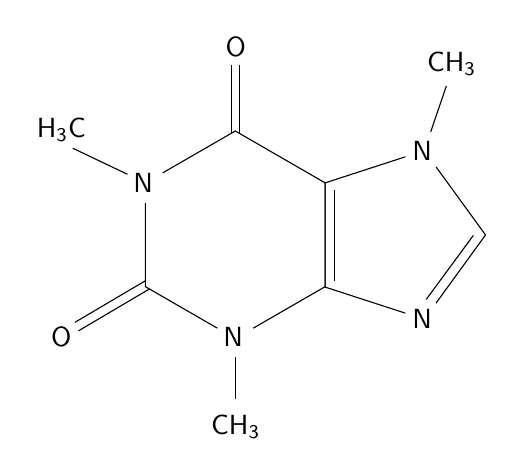
\begin{tikzpicture}[x=0.75pt,y=0.75pt,yscale=-1,xscale=1]
%uncomment if require: \path (0,300); %set diagram left start at 0, and has height of 300

%Shape: Regular Polygon [id:dp004400094577923452]
\draw   (231.6,166.7) -- (188.3,191.7) -- (145,166.7) -- (145,116.7) -- (188.3,91.7) -- (231.6,116.7) -- cycle ;
%Shape: Regular Polygon [id:dp7925754861532168]
\draw   (308.87,141.8) -- (279.36,182.43) -- (231.6,166.91) -- (231.6,116.7) -- (279.36,101.18) -- cycle ;
%Straight Lines [id:da8473227113357105]
\draw    (236,120) -- (236,164) ;
%Straight Lines [id:da21728791560640182]
\draw    (303,142) -- (278,176) ;
%Straight Lines [id:da6777547908917203]
\draw    (145.26,163.7) -- (111,183.92) ;
%Straight Lines [id:da6898565491342596]
\draw    (186.3,60) -- (186.3,92.7) ;
%Shape: Boxed Line [id:dp47917299330626917]
\draw    (145,116.7) -- (110,100) ;
%Shape: Boxed Line [id:dp2519300628036698]
\draw    (279.36,101.18) -- (290,70) ;
%Straight Lines [id:da5432254903819835]
\draw    (188.3,190.9) -- (188.3,220.7) ;
%Straight Lines [id:da998950148390531]
\draw    (147,167.78) -- (112.74,188) ;
%Straight Lines [id:da7607342852654713]
\draw    (190.3,60) -- (190.3,92.7) ;

% Text Node
\draw  [draw opacity=0][fill={rgb, 255:red, 255; green, 255; blue, 255 }  ,fill opacity=1 ]  (145, 116.7) circle [x radius= 9.6, y radius= 9.6]   ;
\draw (145,116.7) node   [align=left] {\begin{minipage}[lt]{8.67pt}\setlength\topsep{0pt}
$\displaystyle \mathsf{N}$
\end{minipage}};
% Text Node
\draw  [draw opacity=0][fill={rgb, 255:red, 255; green, 255; blue, 255 }  ,fill opacity=1 ]  (188.3, 190.9) circle [x radius= 9.6, y radius= 9.6]   ;
\draw (188.3,190.9) node   [align=left] {\begin{minipage}[lt]{8.67pt}\setlength\topsep{0pt}
$\displaystyle \mathsf{N}$
\end{minipage}};
% Text Node
\draw  [draw opacity=0][fill={rgb, 255:red, 255; green, 255; blue, 255 }  ,fill opacity=1 ]  (279.36, 182.43) circle [x radius= 9.6, y radius= 9.6]   ;
\draw (279.36,182.43) node   [align=left] {\begin{minipage}[lt]{8.67pt}\setlength\topsep{0pt}
$\displaystyle \mathsf{N}$
\end{minipage}};
% Text Node
\draw  [draw opacity=0][fill={rgb, 255:red, 255; green, 255; blue, 255 }  ,fill opacity=1 ]  (279.36, 101.18) circle [x radius= 9.6, y radius= 9.6]   ;
\draw (279.36,101.18) node   [align=left] {\begin{minipage}[lt]{8.67pt}\setlength\topsep{0pt}
$\displaystyle \mathsf{N}$
\end{minipage}};
% Text Node
\draw (98.5,88) node   [align=left] {\begin{minipage}[lt]{8.67pt}\setlength\topsep{0pt}
\begin{center}
$\displaystyle \mathsf{H_{3} C}$
\end{center}

\end{minipage}};
% Text Node
\draw (182.5,231) node   [align=left] {\begin{minipage}[lt]{8.67pt}\setlength\topsep{0pt}
\begin{center}
$\displaystyle \mathsf{CH_{3}}$
\end{center}

\end{minipage}};
% Text Node
\draw (286.5,56) node   [align=left] {\begin{minipage}[lt]{8.67pt}\setlength\topsep{0pt}
\begin{center}
$\displaystyle \mathsf{CH_{3}}$
\end{center}

\end{minipage}};
% Text Node
\draw (188.5,51) node   [align=left] {\begin{minipage}[lt]{8.67pt}\setlength\topsep{0pt}
\begin{center}
$\displaystyle \mathsf{O}$
\end{center}

\end{minipage}};
% Text Node
\draw (104.5,191) node   [align=left] {\begin{minipage}[lt]{8.67pt}\setlength\topsep{0pt}
\begin{center}
$\displaystyle \mathsf{O}$
\end{center}

\end{minipage}};


\end{tikzpicture}}
        \caption{Molecular graph.}
        \label{subfig:molecular-graph}
    \end{subfigure}
    \caption{Examples of biological data.}\label{fig:biological-data}
\end{figure*}

Traditional Machine Learning models are designed to work with non-relational real-valued vectors. Thus, they cannot be applied off-the-self to problems where data have a complex structure. In principle, it is possible to circumvent this complexity by hard-coding the relational information into vectors of structural descriptors. While useful to some extent, this approach builds upon a somewhat under-specified representation of knowledge. Moreover, it heavily relies on domain expertise to choose what structural information need to be retained and what need to be discarded. In contrast, Deep Learning methodologies for structured domains allow to extract this relational knowledge directly and in a goal-oriented way. Neural approaches for the recursive processing of structured data have been studied long before the advent of Deep Learning \cite{elman1990rnn,hochreiter1997lstm,sperduti1997generalizedneuron,frasconi1998general} and were generalized to general classes of graph data while modern Deep Learning methods were still under development \citep{micheli2009nn4g,scarselli2009gnn}. These research efforts culminated in three types of neural networks for structured data: Recurrent Neural Networks for sequence data, Recursive Neural Networks for tree/hierarchical data, and Deep Graph Networks for general graph data. Recently, with the availability of large data sources and the increase of computational power, these models have been rediscovered and improved, attracting the attention of researchers coming from very different domains. When applied to challenging biological tasks, these models have demonstrated strong performances and great success
\cite{bianucci2000applicationcascorstructurechemistry,baldi2013recursiveneuralnets,duvenaud2015molecularfingerprint,bradshaw2019moleculechef}.

\section{Objective and Contributions}
The high-level objective of this thesis is to provide the reader with a broad perspective on the kinds of biological tasks that can be tackled with Deep Learning for structured data. We do so by focusing on two classes of learning problems: \emph{predictive} and \emph{generative}. Predictive problems deal with modeling an unknown input-output relationship of interest; generative problems deal with learning the data distribution to sample novel instances. The contributions of this thesis relate to these two general categories.

Relatively to the former, we present two original contributions. The first is an empirical evaluation of different Deep Graph Networks proposed in the literature for graph classification tasks. The second concerns an application of Deep Learning for graphs to the life sciences sub-domain of computational biology. Specifically, we develop a novel learning framework for the prediction of dynamical properties of biochemical pathways with Deep Graph Networks.

As regards the latter, our work consists of two original modeling contributions. The first is a general-purpose, domain-agnostic generative model of unlabeled graphs. The second concerns an application of generative modeling to the life sciences sub-domain of computational chemistry. Specifically, we present a novel generative model of molecules for \emph{de novo} drug design. Following, we discuss our contributions in detail.

\subsubsection*{An Empirical Evaluation of Deep Graph Networks for Graph Classification}
We provide a systematic and fair evaluation of Deep Graph Networks for graph classification tasks. In the literature, these models' evaluation is often biased by poor experimental setups and unfair comparisons. We develop a unified framework under which these models can be evaluated coherently and their results adequately compared. This work lets us also shed light on what Deep Graph Networks learn differently from structure-agnostic baselines and the relation between structural features of the graphs (precisely, the vertex degree) and model performances.

\subsubsection*{A Novel Learning Framework for the Prediction of Dynamical Properties of Biochemical Pathways}
We address a newly formulated predictive problem in the context of biological pathways. A biochemical pathway is a dynamical system in which molecules interact with each other through chemical reactions. Each molecule can take different roles in a biochemical pathway: it can be a reactant, a product of some chemical reaction, and an inhibitor or promoter of other reactions. The system's state corresponds to some function being performed or not (for example, cell replication). Biochemical pathways can be conveniently represented as Petri networks, allowing researchers to study dynamical properties of the system such as reachability of steady states, causality between species, and robustness. Specifically, we focus on the property of robustness, which can be described informally as the pathway's resilience to maintain its function against external perturbations. The standard way to assess robustness requires an extensive number of numerical simulations, which are usually expensive in terms of computational time. We apply Deep Graph Networks to predict robustness indicators on pathways represented as Petri nets, bypassing the need to performing costly simulations. The assumption at the basis of this work is that the structure of the pathway (and not other factors such as kinetic and chemical constants) is sufficient to be effective in this task. We show experimentally for the first time that this is indeed possible to a reasonable extent. Furthermore, we study how different architectural choices of the Deep Graph Network influence performances.

\subsubsection*{A Generative Model for Unlabeled Graph Generation}
Graph generation is a challenging problem with applications in various research fields. We propose a general-purpose recurrent model to generate arbitrary unlabeled graphs, whose structure resembles that of training samples. Despite its conceptual simplicity, we experimentally demonstrate its effectiveness on a wide range of graph datasets. The results show that the model outperforms canonical baselines from graph theory and performs comparably to the current state of the art on unlabeled graph generation.

\subsubsection*{A Generative Model of Molecules for \emph{de novo} Drug Design}
We study the molecular generation problem in the context of \emph{de novo} drug design. Currently, deep generative approaches on this task belong to two broad categories, differing in how molecules are represented. One approach is based on encoding molecular graphs as strings of text and learning a character-based language model on such strings. Another more expressive approach works directly with the molecular graph. The work addresses two limitations of the former generative framework: the generation of invalid or duplicate molecules. To improve validity rates, we develop a language model for small molecular substructures called fragments, loosely inspired by the well-known paradigm of Fragment-Based Drug Design \citep{erlanson2004fbdd}. The proposed architecture generates molecules fragment-by-fragment, instead of atom-by-atom. To improve uniqueness rates, we present a frequency-based masking strategy that helps generating molecules with infrequent fragments. We show experimentally that our model largely outperforms other language model-based competitors, reaching performances comparable to the state of the art in the task. Moreover, we show how the generated samples display molecular properties similar to those of training samples, even in the absence of explicit task-specific supervision.

\section{Structure of the Thesis}
This thesis is divided in four parts. In Part \ref{part:prelimiaries}, we present the necessary introductory notions to facilitate the understanding of the following content. In the first part of Chapter \ref{ch:neural-networks}, we provide a brief overview of the concepts of Machine Learning that are functional to our discussion. The rest of the chapter is dedicated to discuss about the foundations of Neural Networks and Deep Learning for supervised and unsupervised tasks. In Chapter \ref{ch:deep-learning-structures}, we present the class of Deep Learning models for the processing of structured data, namely Recurrent Neural Networks for sequence data, Recursive Neural Networks for tree/hierarchical data, and Deep Graph Networks for graph data. We conclude presenting the framework of Deep Generative Models for graph generation. In Part \ref{part:evaluation-biology}, we present our first two contributions in the context of predictive Deep Learning and its applications to computational biology. Specifically, in Chapter \ref{ch:evaluation-dgns}, we present a fair and rigorous evaluation of existing Deep Graph Networks; while in Chapter \ref{ch:prediction-biochemical-dgn}, we propose a novel application of Deep Graph Networks to the problem of predicting the dynamical properties of biological pathways. Part \ref{part:generative} of the thesis presents our two original contributions in the context deep generative learning of graphs, and its applications to computational chemistry. In Chapter \ref{ch:deep-generative-learning-graphs}, we discuss a general-purpose  model capable of generating unattributed graphs by sequentially generating their edges. In Chapter \ref{ch:deep-generative-learning-drug-discovery}, we introduce a novel generative model of molecules in the context of drug discovery. Lastly, Part \ref{part:fin} concerns concluding remarks and future works, which are discussed in Chapter \ref{ch:conclusions}.

\section{Published Works}
Several publications have contributed to the development of this thesis. Section \ref{sec:dgns} is based on the journal article:

\vspace{1em}
\longfullcite{bacciu2020dgn},
\vspace{1em}

\noindent where we re-elaborated the concepts behind Deep Graph Networks in a systematic introductory review.

\noindent Chapter \ref{ch:evaluation-dgns} draws from our conference paper:

\vspace{1em}
\longfullcite{errica2020fairevaluation},
\vspace{1em}

\noindent which presented a fair and rigorous comparison of several state of the art Deep Graph Networks.

\noindent Chapter \ref{ch:prediction-biochemical-dgn} is a compendium of the work developed in two conference papers:

\vspace{1em}
\longfullcite{bove2020prediction}

\longfullcite{podda2020esannbiochemical}.
\vspace{1em}

\noindent The former work first formulated the predictive problem, receiving the Best Paper Award in the related conference. Later, it has been selected to be extended in a post-proceedings journal publication (in review).

\noindent Chapter \ref{ch:deep-generative-learning-graphs} derives from our work on the conference paper:

\vspace{1em}
\longfullcite{bacciu2019graphesann},
\vspace{1em}

\noindent which was later extended to a journal article in:

\vspace{1em}
\longfullcite{bacciu2020graphgeneration}.
\vspace{1em}

\noindent Lastly, Chapter \ref{ch:deep-generative-learning-drug-discovery} concerns work published in the following conference paper:

\vspace{1em}
\longfullcite{podda2020aistats}.
\vspace{1em}